\documentclass{article}

\usepackage[margin=1in]{geometry} % narrow margins
\usepackage[utf8]{inputenc}
\usepackage[T1]{fontenc}
\usepackage{hyperref}
\usepackage{tabulary}
\usepackage{verbatim}
\usepackage{listings}
\usepackage{graphicx}

%\usepackage{listings}
%\usepackage[cm]{fullpage}
\renewcommand{\labelenumii}{\arabic{enumii}.}
\newcolumntype{P}[1]{>{\centering\arraybackslash}p{#1}}



\title{Project 1 \\ Report \\ INF4121/3121} % Title
\date{\today} % Date for the report
\author{Sebasting Søberg(INF4121) \& Thomas Oddsund(INF3121)}

\begin{document}

\maketitle % Insert the title, author and date

%Requirement 1
\section{\textit{Requirement 1} - Description, analysis and test cases}

	\subsection{Description}
	We are going to review the program Hangman, which derives its name from the game, written in the language Java. The program consists of 5 source files, namely;
	\begin{itemize}
	\item Command.java
	\item FileReadWriter.java
	\item Game.java
	\item HangmanTets.java
	\item Players.java
	\end{itemize}

	\textbf{Command.java} only contains an enumerated type, which contains the possible commands for the program. \textbf{FileReadWriter.java} contains the logic for reading from and writing player objects to file for the scoreboard functionality, as well as a method for sorting and printing the scoreboard. \textbf{Game.java} contains the logic for the game itself, which means handling out, user input, checking input and printing the game dialogue. \textbf{HangmanTets.java} only initializes and starts the Game.java logic. \textbf{Players.java} contains the data structure for a player, as well as methods for fetching name and score.
	%end descrition

	\subsection{Analysis of the testable parts of the program}
	As this program shipped with no requirment, we had to rely on experience and knowledge about the game of hangman to create a model of the flow of the program. This model was based both on our experience, as well as observed behaviour of the program. From this model, we could use black-box technique to design test cases for the program. The test cases were then built as pr. definition, with pre- and post-conditions, inital state, result and steps.
	
	Out previous experience and knowledge helped us in setting up the requirements and model, from which we derived the different test cases. For the test cases, it especially made us set up cases for various forms of input, both valid and invalid, as this is the main vector from which users interact with the system.
\pagebreak

	\subsection{Test cases}
 %Start of test-cases
%Missing test-case for checking number of mistakes is correct?
	\begin{enumerate}
	\setlength\itemsep{1em}

	\item \textbf{Start Hangman}\newline
	\textbf{Initial state:} No program running.\newline
	\textbf{Steps:}
	\begin{enumerate}
	\item Run "java -cp . hangman.HangmanTets" from the folder containing the hangman folder with binaries
	\end{enumerate}
	\textbf{Expected results:} Game displays welcome-statement:
	\begin{lstlisting}[breaklines, gobble=8]
	Welcome to the Hangman game. Please, try to guess my secret word.
	Use 'TOP' to view the top scoreboard, 'RESTART' to start a new game, 
	'HELP' to cheat and 'EXIT' to quit the game.
	The secret word is:  *One-or-more underlines*
	Enter your guess(1 letter allowed):
	\end{lstlisting}
	\textbf{Post condition:} Game awaits input

	\item \textbf{Correct letter entered}\newline
	\textbf{Initial State:} Multiple underlines are displayed in the secret word, more then one unique letter missing.\newline
	\textbf{Steps:}
	\begin{enumerate}
	\item User enters a valid letter X.
	\end{enumerate}
	\textbf{Expected results:} Game displayes the following message; 
	\begin{lstlisting}[breaklines, gobble=8]
	Good job! You revealed 1 letter(s).
	The secret word is: *Current state of secret word,  letter X revealed*
	Enter your guess(1 letter allowed):
	\end{lstlisting}
	\textbf{Post condition:} One or more underlines are replaced with the letter in the correct position, game awaits input.

	\item \textbf{Wrong letter entered}\newline
	\textbf{Initial State:} One or more underlines are displayed in the secret word.\newline
	\textbf{Steps:}
	\begin{enumerate}
	\item User enters an invalid letter X.
	\end{enumerate}
	\textbf{Expected results:} Game displays the following error message: 
	\begin{lstlisting}[breaklines, gobble=8]
	Sorry! There are no unrevealed letters 'X'. 
	The secret word is:  *Current state of secret word*
	Enter your guess(1 letter allowed):
	\end{lstlisting}
	\textbf{Post condition:} The state of the secret word remains unchanged, mistake counter increased by one.

	\item \textbf{Correct letter reveals last letter(no help used)}\newline
	\textbf{Initial State:} One unique letter missing and no help used.\newline
	\textbf{Steps:}
	\begin{enumerate}
	\item User enters a valid letter X
	\end{enumerate}
	\textbf{Expected results:} Game displays the following success-message;
	\begin{lstlisting}[breaklines, gobble=8]
	Good job! You revealed 1 letter(s).
	You won with Y mistake(s).
	The secret word is:  *SECRET WORD*
	Please enter your name for the top scoreboard:
	\end{lstlisting}
	Where Y is the number of unique incorrect letters typed in by the user.\newline
	\textbf{Post condition:}Game ready for input for scoreboard\newline
	
	\item \textbf{Correct number of mistakes(help/no help irellevant)}\newline
	\textbf{Initial State:} One unique letter missing.\newline
	\textbf{Steps:}
	\begin{enumerate}
	\item User enters a valid letter X.
	\end{enumerate}
	\textbf{Expected results:} Game displays the following success-message;
	\begin{lstlisting}[breaklines, gobble=8]
	Good job! You revealed 1 letter(s).
	You won with Y mistake(s).
	The secret word is:  *SECRET WORD*
	\end{lstlisting}
	Where Y is the \textbf{correct} number of unique incorrect letters typed in by the user.\newline
	\textbf{Post condition:} Game ready for input for scoreboard.

	\item \textbf{Single non-alphabetic character}\newline
	\textbf{Initial State:} Game running, awaiting input.\newline
	\textbf{Steps:}
	\begin{enumerate}
	\item Users enters a non-alphabetic character.
	\end{enumerate}
	\textbf{Expected results:} Game ignores input, asks for new character.\newline
	\textbf{Post condition:} Game awaits input.

	\item \textbf{Multiple characters entered}\newline
	\textbf{Initial State:} Game running, awaiting input.\newline
	\textbf{Steps:}
	\begin{enumerate}
	\item User enters multiple characters.
	\end{enumerate}
	\textbf{Expected results:} Game ignores input, asks for a new character.\newline
	\textbf{Post condition:} Game awaits input.

	\item \textbf{Help command}\newline
	\textbf{Initial State:} Game running and awaiting user input.\newline
	\textbf{Steps:}
	\begin{enumerate}
	\item User enters "help"
	\end{enumerate}
	\textbf{Expected results:} One letter is revealed in the secret word. help flag set for user in this game.\newline
	\textbf{Post condition:} Help flag is set on user, game awaits user input.\newline

	\item \textbf{Correct letter reveals last letter(help used)}\newline
	\textbf{Initial State:} One unique letter missing and help used.\newline
	\textbf{Steps:}
	\begin{enumerate}
	\item User enters a valid letter X.
	\end{enumerate}
	\textbf{Expected results:}
	\begin{lstlisting}[breaklines, gobble=8]
	Good job! You revealed 1 letter(s).
	You won with Y mistake(s). but you have cheated. You are not allowed to 
	enter into the scoreboard.
	The secret word is:  *SECRET WORD*
	\end{lstlisting}
	Where Y is the number of unique incorrect letter typed in by the user.\newline
	\textbf{Post condition:} Game restarts, then displays welcome statement and awaits input.\newline

	\item \textbf{Restart command}\newline
	\textbf{Initial State:} Game running and awaiting user input.\newline
	\textbf{Steps:}
	\begin{enumerate}
	\item User enters "restart"
	\end{enumerate}
	\textbf{Expected results:} The game starts a new game.\newline
	\textbf{Post condition:} New game with a new word running, game awaits user input.\newline

	\item \textbf{Exit command}\newline
	\textbf{Initial State:} Game running and awaiting user input.\newline
	\textbf{Steps:}
	\begin{enumerate}
	\item User enters "exit"
	\end{enumerate}
	\textbf{Expected results:}Game exits\newline
	\textbf{Post condition:}No game running\newline

	\item \textbf{User enters name for scoreboard}\newline
	\textbf{Initial State:} User have guessed the correct word without the help command.\newline
	\textbf{Steps:}
	\begin{enumerate}
	\item User guesses the correct word
	\item User inputs name for scoreboard
	\end{enumerate}
	\textbf{Expected results:} Name+score stored in records, new game started\newline
	\textbf{Post condition:} Scoreboard has one new entry containing the playername + score, and a new game has started.\newline

	\item \textbf{Top command}\newline
	\textbf{Initial State:} Game running and awaiting user input.\newline
	\textbf{Steps:}
	\begin{enumerate}
	\item User enters "top"
	\end{enumerate}
	\textbf{Expected results:} Game displays the scoreboard and starts a new game.\newline
	\textbf{Post condition:} Game awaits user input.\newline
	\end{enumerate}

	\textbf{Non-functional testing}
	After some discussion we realized that some factors in non-functional testing
	are of importance. Namely:
	\begin{enumerate}
		\item
		\textbf{Performance}
		The performance of the program can be tested. Since this is supposed to be a rather simple program,
		a few things to test can be that it handles input fast enough(i.e. that it prints out correct/incorrect, and that it's ready
		for new input within a set time) and that it uses minimal amount of memory(i.e. locked device where it runs in a continuous
		loop can lead to a stack overflow if it continuously instantiates new classes in the wrong way).
		\begin{comment}
		After each game "round" the program calls: new Game()
		which can be a performance bottleneck whereas one plays
		this game several million times. This can happen in situations
		where this program are loaded onto a locked device for playing.
		So instead of calling new Game() one should simply call a startMethod instead.
		And move the internal statements in the constructor over in that method so we 
		avoid having multiple Games on the stack which increases space requirements.
		\end{comment}

		\item
		\textbf{Maintainability}
		All systems, even a small and easy one, should be properly documented, via comments, names of variables, method names
		etc. It probably isn't necesearry with a huge document base for a project of this size, but for maintainability in the future,
		the program should have the proper amount of comments, and proper names on variables, methods etc.
		\begin{comment}
		The system is poorly documented and the statements is not intuitively named everywhere.
		There are also some methods which doesn\'t do anything except increasing the complexity of
		the program. Also there are places where exceptions are caught individually without any
		purpose. And all of this makes the code harder to analyze and or change.
		\end{comment}

	\end{enumerate}


 %End of test-cases

%Requirment 2
\section{\textit{Requirement 2} - Metrics at project and file level}

\subsection{Metrics at project level}

%metrics at project level
\begin{tabulary}{1.0\textwidth}{| P{3cm} | P{2.7cm} | p{8.5cm} |}
	\multicolumn{3}{c}{\textbf{Metrics summary}} \\ \hline
	\textbf{Parameter} & \textbf{Value} & \textbf{How are the values} \\ \hline 
	Files & 5 & Based on the name of the files and the size of the project, this
	seems like a good split.\\ \hline
	Lines & 441 & We can't really say much about this value, as it relies on the
	logic in the application.\\ \hline
	Statements & 222 & Same as above, relies on the logic of the application and 
	how the classes/methods are set up.\\ \hline
	Percent Branch Statements & 18.5 & Same as above, this relies entirely on
	the logic of the application, and can be quite hard to abstract away.\\ \hline
	Method Call Statements & 147 & This might seem somewhat high, based on the number
	of "Classes and Interfaces" and "Methods per Class".\\ \hline
	Percent Lines with Comments & 5.2 & According to the Kivat graph, this seems low, 
	and is an indication of poorly documented code. \\ \hline
	Classes and Interfaces & 5 & Depends on the logic of the application, hard to
	say anything about.\\ \hline
	Methods per Class & 4,20 & Seems like a good number in itself, but if we also
	account for number of "Classes and Interfaces" as well as "Method Call Statements",
	this number might indicate that the project could benefit from refactoring methods.\\ \hline
	Average Statements per Method & 8,14 & This number seems pretty good according
	to the kivat graph. \\ \hline
	Name of Most Complex Method & Game.findLetter AndPrintlt() & This just shows us
	where we can start our initial work for refactoring.\\ \hline
	Maximum Complexity & 12 & This number seems pretty high, and indicates that the 
	method in question(findLetterAndPrintIt()) might need some serious refactoring.\\ \hline
	Maximum Block Depth & 9+ & This is another number which seems rather high, and 
	indicates that at least one code has an unnecessary amount of nested statements,
	probably via execution control statements.\\ \hline
	Average Block Depth & 2,90 & This seems a bit high, and may indicate that the
	code has for example too few methods or too many if-statements.\\ \hline
	Average Complexity & 2,95 & Average complexity seems fine, so the high complexity
	and depth number may indicate that a subset of all methods needs refactoring, since
	the program overall is fine.\\ \hline
	Line Number of Most Complex Method & undefined & This is more of a per-file value.\\ \hline
	Line Number of Deepest Block & undefined & Another per-file value. \\ \hline
\end{tabulary}
\pagebreak

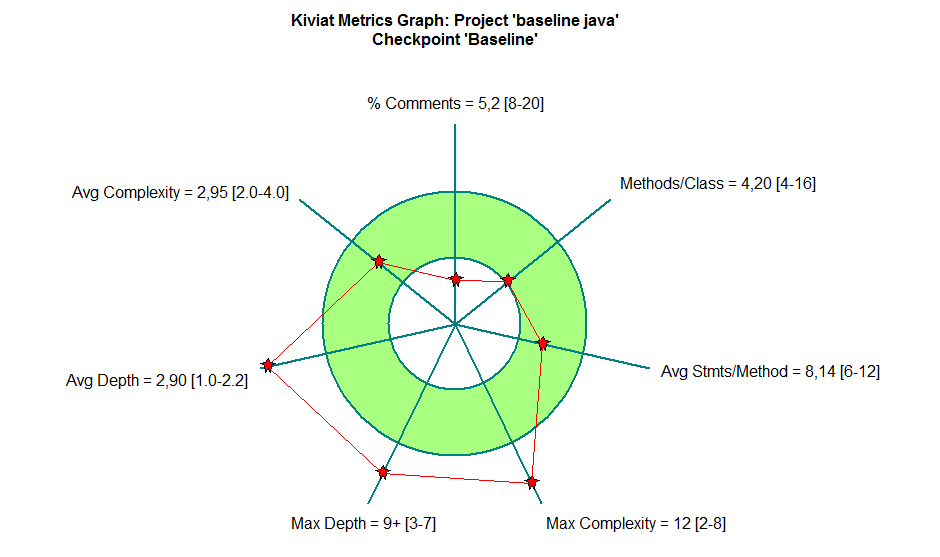
\includegraphics[width=0.9\textwidth]{Hangman-Kiviat-before.png}

\textbf{Comments on the numbers}\newline

We think that \textit{Comments, Max Complexity, Max Depth and Avg Depth}
need to change. Also, \textit{Method Call Statements} and/or \textit{number of methods} might need some work.
 This is based on the Kivat graph and the numbers overall. 22(5.2\%) lines of comments seems
  rather low to ensure good documentation, max complexity and max depth of 12 indicates that
   at least one method does too much work, while average depth indicates that one or more
    methods contains too many nested statements. The ratio of method call statements(147)
     to number of methods(4.20 * 5 = 21) also seems somewhat off, and this number(like max
      complexity/max depth) might indicate that one method does too much work, or that methods
       for doing some aggregated work is missing.


To answer the rest of the questions; the biggest file by the number of lines is
 fileReadWriter.java with 219 lines, the file with the most branches is fileReadWriter.java
  where the branches stands for 20,8 \% of the file. The file with the most complex code is
   Game.java. The metrics used for this conclusion is Max complexity and Average Statements
   per method, where Game.java's score here was 12 and 11.57. 

\subsection{Metrics at file level}
\vspace {0.10 cm}
\begin{center}
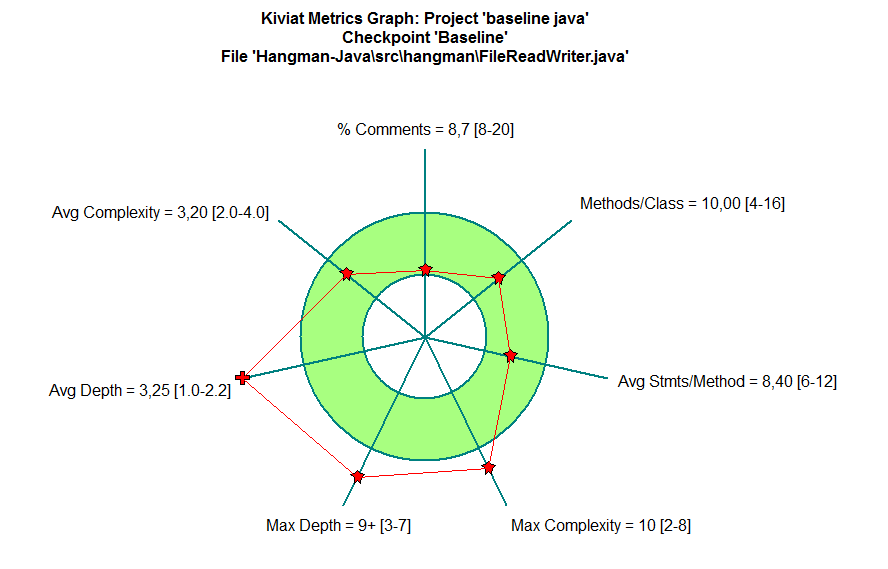
\includegraphics[width=0.9\textwidth]{FileReadWriter-kiviat-before.png}
\end{center}
\begin{enumerate}
\item
How do you interpret the metrics applied on your file? How are they different the metrics you
obtained on the whole project, compared with the metrics on this file?\newline
\textbf{We chose FileReadWriter.java}\newline
We interpret FileReadWriter as more complex then the average for the project, as the 
numbers for average complexity and average depth are higher. Its number for max complexity and
max depth is also pretty high. At the same time, it looks like it's more commented then
the average of the project, which is good, and with another look at the numbers, it contains 
almost all of the comments in this project. But the average complexity, average statements
pr method and the number of method seems well balanced.

%Project vs FileReadWriter.java
\item
Would	you	refactor	(re-write)	any	of	the	methods you	have	in	this	file?	

\begin{tabulary}{0.5\textwidth}{| c | c | c | c | c |}
 \hline
\textbf{Method names} &	\textbf{Complexity} & \textbf{Statements} & \textbf{Max Depth} & \textbf{Calls} \\ \hline

addRecords()				& 2 & 6 & 3 & 3 \\ \hline
closeFileFromReading() 		& 1 & 1 & 2 & 1 \\ \hline
closeFileFromWriting() 		& 3 & 5 & 4 & 3 \\ \hline
nop() 				  		& 1 & 15 & 10 & 15 \\ \hline
oldReadRecords()		  	& 1 & 5 & 2 & 5 \\ \hline
openFiletoRead()			& 3 & 5 & 5 & 2 \\ \hline
openFileToWite()			& 2 & 3 & 3 & 2 \\ \hline
printAndSortScoreBoard()	& 10 & 24 & 8 & 32 \\ \hline
readRecords()				& 6 & 13 & 7 & 8 \\ \hline
tryCloseFileFromReading()	& 3 & 7 & 4 & 4 \\ \hline
\end{tabulary}

Based on the numbers overall and for each method, most definitely:
\begin{enumerate}
\item
closeFileFromReading() because it only has one statement, which looks like a function call.
Its name might also indicate that it does the same as tryCloseFileFromReading().

\item
nop() has 15 statements, whom are all system calls(based on the number), and a max depth
of 10. Based on the numbers, this might be a rather useless method, unless it contains
some sort of control flow, but based on the number of methods and its name, it is highly unlikely.

\item
oldReadRecords() might be deprecated method based on its name, since another method called addRecords() exists. It also contains only 5 statements, where all are system calls, so this is another method where its relevance is doubtful at best.
\begin{comment}
oldReadRecords() calls readRecords() 5 times. But for no apperent reason.
This is undefined behavior because it doesnt check of many records that eventually
would've been stored. It has the same problem as nop(), it is private and nothing else in this class is using it so it is rubbish.
\end{comment}

\item
printAndSortScorebard() has more calls then statements, which might indicate that it's not optimized or does something rather clunky.

\end{enumerate}

Do note that this list is only based on the metrics retrieved by SourceMonitor, and only contains those that clearly stood out. When the optimization begins, other methods may be touched if they are found to contain unusable/unnecessary code, badly optimized code etc.

\end{enumerate}
%Requirement 3
\section{\textit{Requirement 3} -Improvements based on metrics}

\subsection{Identified metrics at project level that needs improvment}
\textbf{Comments, Max Complexity, Max Depth and Avg Depth} are metrics that really need to be improved, as comments are very low, while the rest are very high. Methods/Class also seems somewhat low, and might be something that will naturally increase as we deal with the first four listed parameters.

\subsection{Examples of refactored/improved code}
%Both list of code files, link to github public repo and specific cases
\begin{enumerate}
	\item
	\textbf{FileReadWriter.java}
	FileReadWriter has two which are never called and therefor removed nop() and oldReadRecords()
	respectively.
	closeFileFromReading() just calls tryCloseFileFromReading() so that one is removed.
	printAndSortScoreBoard() tries to print out results two times and sort the list two times.
	The whole method is changed and now only contains a loop of the ArrayList myArr which is sorted
	with collections.sort(). This works since Players.java has implemented Comparable<Players>.
	And instead of having one method to open read/write and close I refactored all of these methods
	sequences of operations to one for open, writing and closing and the same for open reading and closing. This is mainly achieved due to the use of try-with-resources which saves a lot of space and
	makes closing method unnecessary in the whole file. 
	\textbf{Example from FileReadwriter \textit{opening file, writing to it and closing} :\newline}
	\hspace*{-2.0cm}\begin{tabulary}{0.5\textwidth}{| c | c |}
	 \hline
	 Before & after \\ \hline
	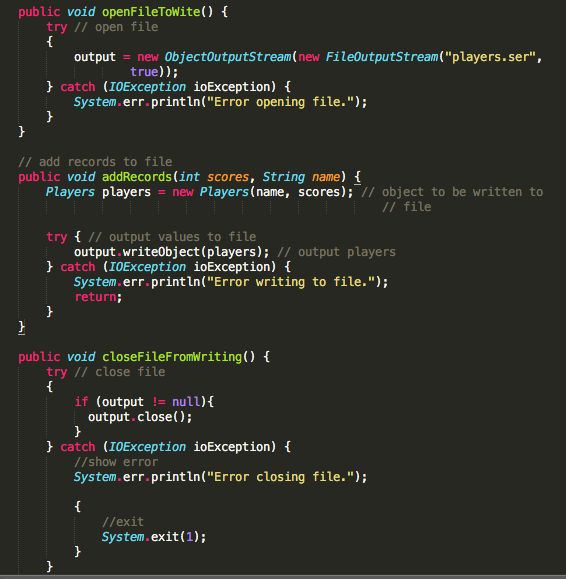
\includegraphics[scale=0.4]{FileReadWriter-EXAMPLE-BEFORE.png} & 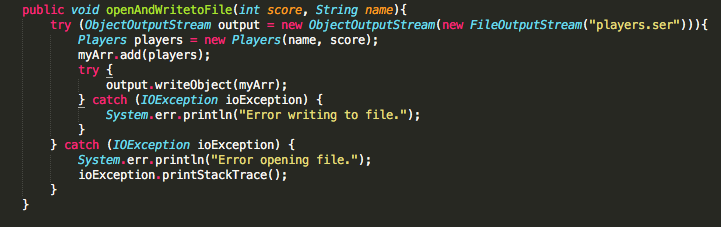
\includegraphics[scale=0.4]{FileReaderWriter-EXAMPLE-AFTER.png} \\ \hline
	\end{tabulary}

	\item
	\textbf{Players.java}
	Comments are added for explaining the implementations for Serializable and Comparable<Players>.
	The method CompareTo is overrided so sorting can be done with the trivial Collections.sort() method. \textit{Why invent the wheel if is already exists?} % du kan fjerne denne om du vil, men tror Raluca kanskje setter pris på den. :p
	\item
	\textbf{HangmanTets.java}
	This file is erased, because the only thing it does is making a reference to Game.java and calling the start method there. This is moved to Game.java. One file less that actually does practically nothing.
	\item
	\textbf{Game.java}
	First of all we moved the logic from HangmanTets.java here so it got it's own main method which starts the game, and we cleaned up some unnecessary blocks and statements. Next, we
	created a class called runHangman, in which we placed initialization of class variables
	which needed changing between games. Thus, we greatly simplified the constructor, and
	eliminated a potential problem where stack overflow might occur due to too many games
	started. As the getRandWord and getW were simple methods for setting two class variables, they were also eliminated since we could simplify them into one-line statements. When it comes to the method running the game, called findLetterAndPrintIt(),
	we did a whole lot of refactoring. Firstly, we changed the name to gameLoop, as the name
	was more describing. Secondly, we moved a whole lot of code into seperate methods. Checking
	if the input consists of help was moved to the commandCheckAndExecute(former menu)-method, 
	were the rest of the commands were handled, the input-loop were moved to a method called
	inputLoop and checking the input for correctness(replacing dash with letter and countning 
	number of correct characters) was moved to a method called 
	replaceDashes(). This resulted in cleaner and more understandable code which has methods
	whose focus lies on one thing.

	\item% Er du uenig? Vi kan fint flytte den inn Game.java og slette hele filen?
	% http://www.coderanch.com/t/385256/java/java/Package-Enums
	% eneste nyttige jeg fant om det.
	\textbf{Commands.java}
	We decided to keep this in it's own file to have more readable code. Although Game.java is the only one the commands. Having it in it's own file empowers the OO-programming scheme.

\end{enumerate}


\subsection{New metrics at project level vs old} % just use kiviat graphs here?
\hspace*{-0.5cm}
\begin{tabulary}{0.5\textwidth}{| c | c |}
 \hline
Without filereadwriter.java & With filereadwriter.java \\ \hline
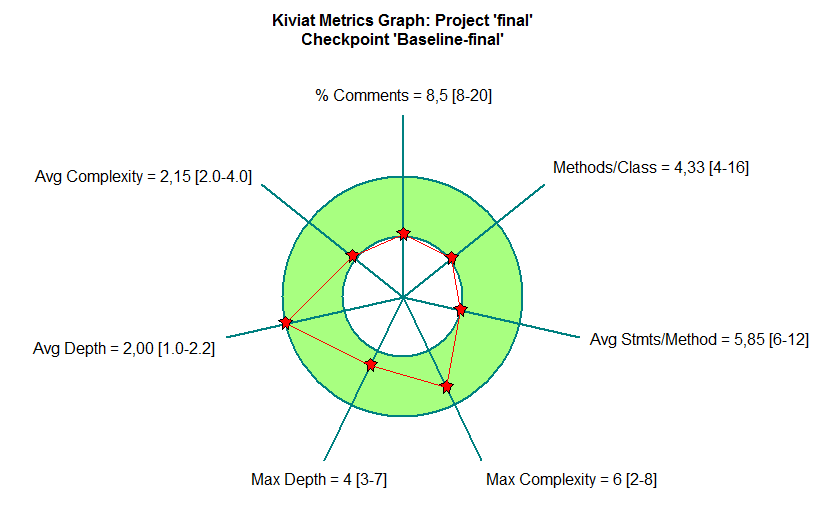
\includegraphics[scale=0.4]{Project-after-with-filereadwriter.png} & 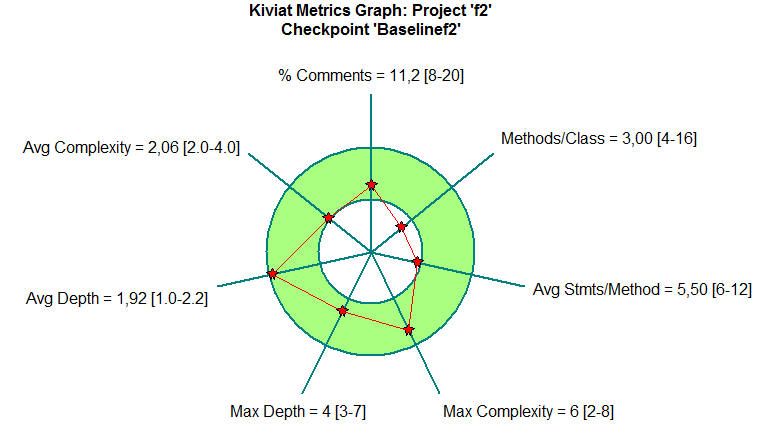
\includegraphics[scale=0.4]{Kiviat-project-without-filereadwriter.png} \\ \hline
\end{tabulary}\vspace{0.2cm}

The problem here is that Sourcemonitor doesn't count classes correctly, try-with-resources is not supported in Sourcemonitor and is regarded as classes not try's with a statement. So it alo misses the statement count for whatever's inside the try. Therefor Methods/class, avg Stmts/Method is not counted correctly. So if we count statements and classes ourself the score for FileReadWriter is:
\textit{Methods/class: 3 Avg and Stmts/methods: 6.7)} and this together with the rest of the project adds up to: \textit{Methods/class: 4.33+3/2=3.6 Avg and Stmts/methods: 6.7+5.50/2=6.1)}
So the only number we havent sufficiently achieved is Methods/class this is commented in detail in remarks.

\subsection{New metrics at file level vs old} % just use kiviat graphs here?
\begin{enumerate}
	\item
	\textbf{FileReadWriter.java}
	In FileReadWriter.java:\newline
	\textit{Avg Stmts/methods Methods/class} must be calculated individually, due to the lack
	of support for newer datastructures.

	In FileReadWriter.java we have 20 statements and 3 methods which 
	rounded up is 6.7 statements per method and 3 methods per class.\newline
	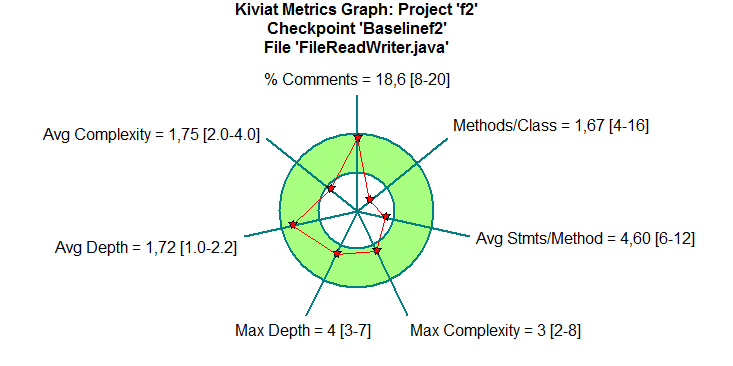
\includegraphics[scale=0.5]{Kiviat-filereadwriter-after.png}\newline

	\item
	\textbf{Game.java}

	\item
	\textbf{Players.java} % gidder du å legge inn en kiviat graf her? hakke tilgang til windows akkurat nå.


	\item%remove this if you choose not to have it in a separate file
	\textbf{Command.java}

\end{enumerate}


\subsection{Github link}
\href{https://github.com/thomaco/INF3121-oblig1}{\textbf{https://github.com/thomaco/INF3121-oblig1}}

\subsection{Remarks and Conclusion}% skal renskrive det her imorgen!
\textbf{Sourcemonitor calculation\newline}
Sourcemonitor doesn't count statements that are separated
by try-catch or nested try-catches even though they are guaranteed to be
executed. 
Sourcemonitor also struggles with newly implemented 'syntatic' sugars and so forth like
try with resources. We have to take all of this into consideration when reading these numbers.
This is also the reason why we chose to show the result of the new project both with and without it.
Also this is a decision the developers of Sourcemonitor has taken and as long as you are aware of this fact and consider this you will be fine. \newline
When sourcemonitor caluclates your comments it only calculated how many lines are either \textbackslash \textbackslash or \textbackslash* * *\textbackslash not if there is some text there. I mean this misguides especially if one is a fan of the neat \textbackslash* * *\textbackslash syntax for writing code.


\textbf{Explaination of FileReadWriter\newline}
Here we had to make a choice between which metric we wanted to satisfy -
Avg Stmts/methods or Methods/class. We chose Avgs Stmts/Methods since
more Methods meant that we would increase average depth. The choice
came from the fact that if we fulfill Avg Stmts/Methods, then
Methods/Class goes under four, but if we satisfy Methods/Class, then
Avg Stmts/Methods goes under 4.33. So it came to a choice between
5 methods with only 3-4 statements in each method, or 3 methods with
around 7 statements in each. \newline\newline
\begin{comment}
Avg Stmts/methods vs Methods/class
chosed Stmts/methods since Methods/class
also would've increased avg depth over 2.0
so basically instead of having two over we only have one.
The problem here is that if we fulfill Stmts/methods then Methods/class
goes < 4 but if we satisfy Methods/class then Stmts/methods < 4.33.

Either 3 or 5 methods for FileReadWriter.java also per class
with only 3-4 statements in each or 3 methods with 7 statements
in each method. 
\end{comment}
So in order to get the metrics inside the green area we would have to
write meaningless code statements in order to get our statement per method up,
or have extra methods to get that ratio up which isn't particularly useful. Our
methods contains exactly what they need to contain in order to do their job. Sourcemonitor
thinks this is too small some places, but those numbers are only omnious. 
This is the time to keep in mind that Sourcemonitor only is \textit{indicative}
and not conclusive, actually far from it. It is only a small part of the analytics
that should be done when analyzing code for optimization. 


\begin{comment}
make a couple of remarks about how easy or not it was for you to maintain the code
(to modify it in order to improve it). Is there anything that you would have done differently on
the ini'al code to make its maintenance easier?
\end{comment}

\end{document}